\documentclass[a4paper,10pt]{article}

\usepackage[utf8]{inputenc}
\usepackage[T1]{fontenc}
%\usepackage[francais]{babel}
\usepackage{amsmath,amsfonts}
\usepackage{graphicx}
\usepackage{dsfont}
\usepackage{fancyvrb}
\usepackage{enumitem}
\usepackage[top=2cm, bottom=2.5cm, left=3cm , right=3cm]{geometry}

\renewcommand{\baselinestretch}{1.1}

\newcommand{\var}{\mbox{var}}
\newcommand{\E}{\mbox{E}}
\newcommand{\Disk}{\mathcal{D}}   

\begin{document}
\begin{center}
\hrule \vspace{3mm}
	{\Large Exam : Statistical modelling and its applications}\\ \vspace{3mm}
	{Mines Saint-\'Etienne -- 21 Décembre 2016} \\  \vspace{2mm}
	{\footnotesize No document allowed except the Gaussian process regression handout, the slides of the \\ optimization lecture and an A4 sheet with hand written notes. The scoring scale indicated for each question and exercise is only an indication, it may be adapted for the final grading. }\\ \vspace{3mm}
	\hrule
\end{center}
\vspace{5mm}

%%%%%%%%%%%%%%%%%%%%%%%%%%%%%%%%%%%%%%%%%%%%%%%%%%%%%%%%%%%%%%%%%%%%
%%%%%%%%%%%%%%%%%%%%%%%%%%%%%%%%%%%%%%%%%%%%%%%%%%%%%%%%%%%%%%%%%%%%
\subsection*{Exercise 1 : The Morris method \hfill [2 pts]} 

Let $f_1,\ \dots \ ,\ f_6$ be six functions over $[-\frac{1}{2}, + \frac{1}{2}]$ defined as:
\begin{align*}
f_1 \left(x_1, x_2 \right) &= x_1^2 + x_2^2 & f_2 \left(x_1, x_2 \right) &= x_1 + 2 x_2 + 2x_1 x_2  \\  
f_3\left(x_1, x_2 \right)&= \left(x_2 + 1\right)^2 & f_4 \left(x_1, x_2\right)&= x_1\left(1+x_1\right) \\  
f_5 \left(x_1, x_2 \right) &= x_1 - 2 x_2 + 2x_1^2 & f_6 \left(x_1, x_2 \right) &= 1+ 2 x_1 - x_2.
\end{align*}

\noindent
For four of these functions, we apply the Morris method ($r = 20$ repetitions) and we obtain the following graphs for the averages $\mu^\ast$ and the standard deviations $\sigma$ of the absolute finite differences: 
\begin{center}
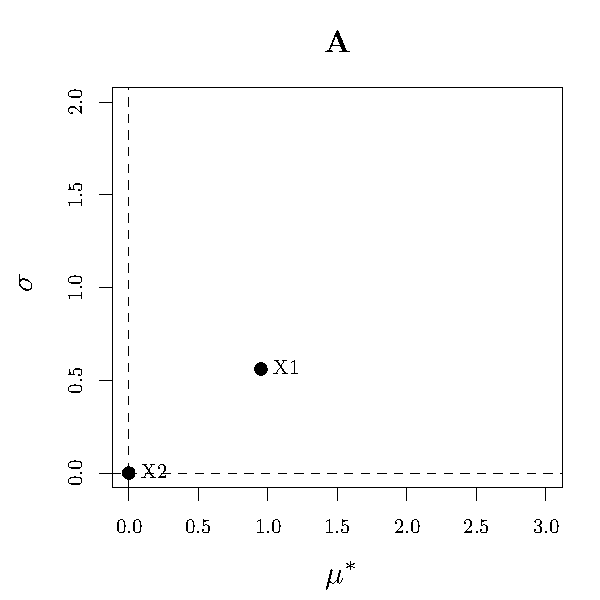
\includegraphics[width=6cm]{figures/exo_morris1.pdf}\qquad
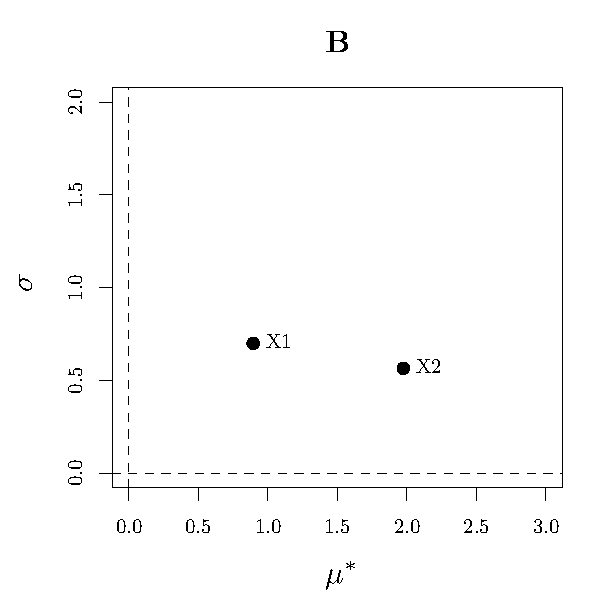
\includegraphics[width=6cm]{figures/exo_morris2.pdf}\\ \ \\
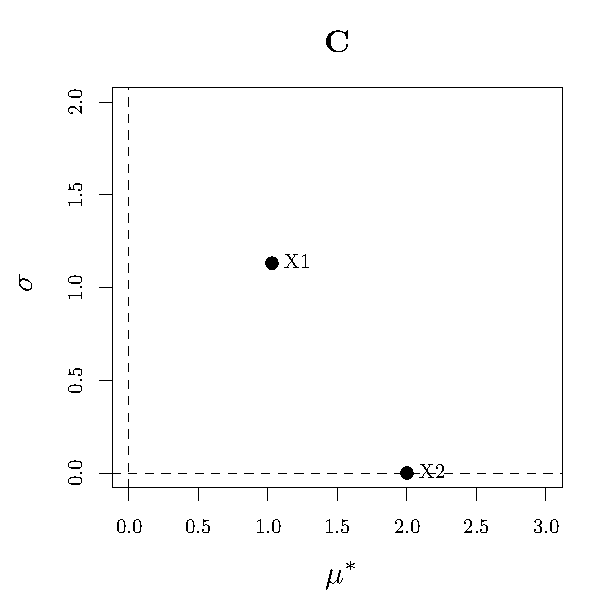
\includegraphics[width=6cm]{figures/exo_morris3.pdf}\qquad
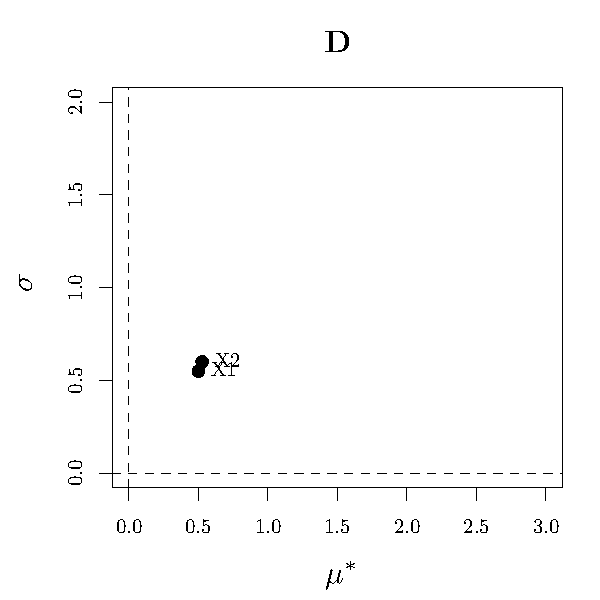
\includegraphics[width=6cm]{figures/exo_morris4.pdf}
\end{center}

\noindent
\begin{enumerate}[label=Q\arabic*.]
  \item {[2 pts]} Can you recover the functions associated to each graph? Justify briefly your answers.
\end{enumerate}

%%%%%%%%%%%%%%%%%%%%%%%%%%%%%%%%%%%%%%%%%%%%%%%%%%%%%%%%%%%%%%%%%%%%
%%%%%%%%%%%%%%%%%%%%%%%%%%%%%%%%%%%%%%%%%%%%%%%%%%%%%%%%%%%%%%%%%%%%
\newpage
\subsection*{Exercise 2 : Sobol-Hoeffding decomposition over the disk \hfill [2 pts]}

Let $\Disk = \lbrace\left( x, y \right) \in \mathbb{R}^2, x^2 + y^2 \leq 1\rbrace$ be the unit disk in Cartesian coordinates and $X = \left(X_1, X_2\right)$ a random point, uniformly distributed over $\Disk$. We are interested in performing sensitivity analysis on the following function:
\begin{equation*}
  f(x_1,x_2) = x_1 + \sqrt{x_1^2 + x_2^2}.
\end{equation*}

\begin{enumerate}[label=Q\arabic*.]
\item {[1 pt]} Explain geometrically (based on a graphic for instance) that:
\begin{equation*}
  \begin{cases}
  \mathbb{E} \big(X_2 \vert X_1 = \frac{3}{4} \big) = \mathbb{E} \big(X_2 \vert X_1 = \frac{1}{4}  \big), \\
  \mathrm{var} \big(X_2 \vert X_1=\frac{3}{4} \big) < \mathrm{var} \big(X_2 \vert X_1 = \frac{1}{4}\big). 
  \end{cases}
\end{equation*}
As a consequence, is it possible to perform Sobol sensitivity analysis directly on $f$ ? 
\item {[1 pt]} We now consider the polar representation of $f$:
\begin{equation*}
  f_p(\rho,\theta) = \rho \cos(\theta) + \rho \, ,
\end{equation*}
and we denote by $R$ and $A$ two independent random variables over $[0, 1]$ and $[0, 2\pi)$ and we use the following notations: 
$m_r = \mathbb{E} \big(R\big)$, $m_a = \mathbb{E} \big(\cos(A) \big)$. What is the Sobol decomposition of $ f_p$ ? The result can be expressed as a function of $m_r $ and $m_a$. 
\item[\textbf{bonus:}] We now assume that $\big(R \cos(A), R \sin(A) \big)$ is uniformly distributed on the disk. What is the distribution of $A$? Compute the cumulative distribution function (la fonction de répartition) of $R$. Deduce the associated values of $m_a$ and $m_r$.
\end{enumerate}

%%%%%%%%%%%%%%%%%%%%%%%%%%%%%%%%%%%%%%%%%%%%%%%%%%%%%%%%%%%%%%%%%%%%
%%%%%%%%%%%%%%%%%%%%%%%%%%%%%%%%%%%%%%%%%%%%%%%%%%%%%%%%%%%%%%%%%%%%
\subsection*{Exercise 3 : Polynomial Chaos \hfill [4 pts]}
We consider the uniform probability measure on $[-1,1]$ and the Legendre basis which consists in orthonormal polynomials for $L^2$ with increasing orders:
\begin{equation*}
  \begin{split}
    h_{0}(x) & = 1 \\
    h_{1}(x) & = \sqrt{3}\ x \\
  \end{split}
  \qquad \qquad \qquad 
  \begin{split}
    h_{2}(x) & = \sqrt{5}/2 (3x^2 -1) \\
     & \dots 
  \end{split}
\end{equation*}

\begin{enumerate}[label=Q\arabic*.]
\item {[1 pt]} Detail how to compute the next basis function $h_3$ and give its expression.
\item {[1 pt]} We now consider the following basis of functions over $[-1,1]^2$: 
\begin{equation*}
  \begin{split}
    h_{00}(x) & = h_{0}(x_1) \times h_{0}(x_2) \\
    h_{10}(x) & = h_{1}(x_1)\times h_{0}(x_2)\\
    h_{01}(x) & = h_{0}(x_1) \times h_{1}(x_2) \\
  \end{split}
  \qquad \quad
  \begin{split}
    h_{11}(x) & = h_{1}(x_1) \times h_{1}(x_2) \\
    h_{20}(x) & = h_{2}(x_1)\times h_{0}(x_2) \\
    h_{21}(x) & = h_{2}(x_1)\times h_{1}(x_2) \\
  \end{split}
  \qquad \quad
  \begin{split}
    h_{02}(x) & = h_{0}(x_1) \times h_{2}(x_2) \\
    h_{12}(x) & = h_{1}(x_1)\times h_{2}(x_2) \\
    h_{22}(x) & = h_{2}(x_1)\times h_{2}(x_2) \\
  \end{split}
\end{equation*}
Show that these basis functions are orthonormal for a uniform probability measure on $[-1,1]^2$. Deduce that these functions are centred and satisfy the Sobol non simplification conditions.
\item {[2 pt]} Let $f$ be a function over $[-1,1]^2$, and let $X$ be a set of 20 points in $[-1,1]^2$ for which the value of $f$ is known: $f(X)=F$. We denote by $\beta$ the vector of the coefficients of a linear regression model based on these observations and the above basis:
\begin{equation*}
 m(x) = \sum_{0 \leq i,j \leq 2} \beta_{i,j} h_{i,j}(x).
\end{equation*}
What is the Sobol decomposition of $m$. Compute the Sobol indices of $m$, your result should be expressed as a function of the $\beta_{i,j}$.
\end{enumerate}

%%%%%%%%%%%%%%%%%%%%%%%%%%%%%%%%%%%%%%%%%%%%%%%%%%%%%%%%%%%%%%%%%%%%
%%%%%%%%%%%%%%%%%%%%%%%%%%%%%%%%%%%%%%%%%%%%%%%%%%%%%%%%%%%%%%%%%%%%
\newpage
\subsection*{Exercise 4 : Kriging models \hfill [2 pts]}
You will find bellow the descriptions and the graphs of various models. Can you recover which graph is associated with each model? Justify briefly your answers.\\

\hspace{-1.2cm}\begin{minipage}[t]{4.3cm}
\underline{Model 1}
\footnotesize
\begin{Verbatim}
Trend  coeff.:
                       
 (Intercept)     0.0000

Covar. type  : matern5_2 
Covar. coeff.:
                       
    theta(x)     0.3000

Variance: 9

Nugget effect : 0.2
\end{Verbatim}
\end{minipage}
\begin{minipage}[t]{4.3cm}
\underline{Model 2}
\footnotesize
\begin{Verbatim}
Trend  coeff.:
                       
 (Intercept)     0.0000
           x     6.0000

Covar. type  : gauss 
Covar. coeff.:
                       
    theta(x)     0.1000

Variance: 9

Nugget effect : 0
\end{Verbatim}
\end{minipage}
\begin{minipage}[t]{4.3cm}
\underline{Model 3}
\footnotesize
\begin{Verbatim}
Trend  coeff.:
                       
 (Intercept)     0.0000

Covar. type  : gauss 
Covar. coeff.:
                       
    theta(x)     0.0200

Variance: 4

Nugget effect : 0
\end{Verbatim}
\end{minipage}
\begin{minipage}[t]{4.3cm}
\underline{Model 4}
\footnotesize
\begin{Verbatim}
Trend  coeff.:
                       
 (Intercept)     0.0000

Covar. type  : exp 
Covar. coeff.:
                       
    theta(x)     0.3000

Variance: 9

Nugget effect : 0
\end{Verbatim}
\end{minipage}
\medskip
\begin{center}
  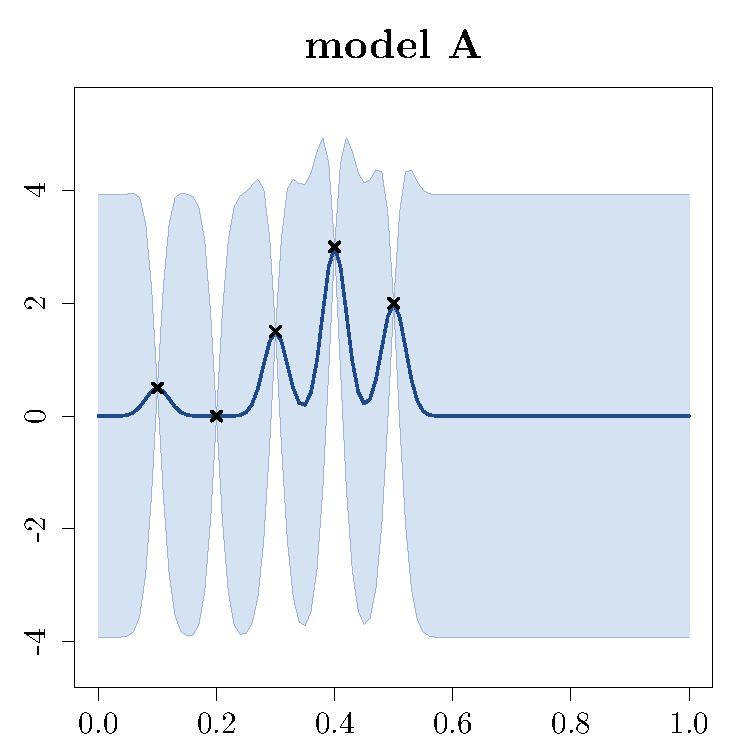
\includegraphics[width=4.6cm]{figures/exo_kriging_3.pdf}\quad 
  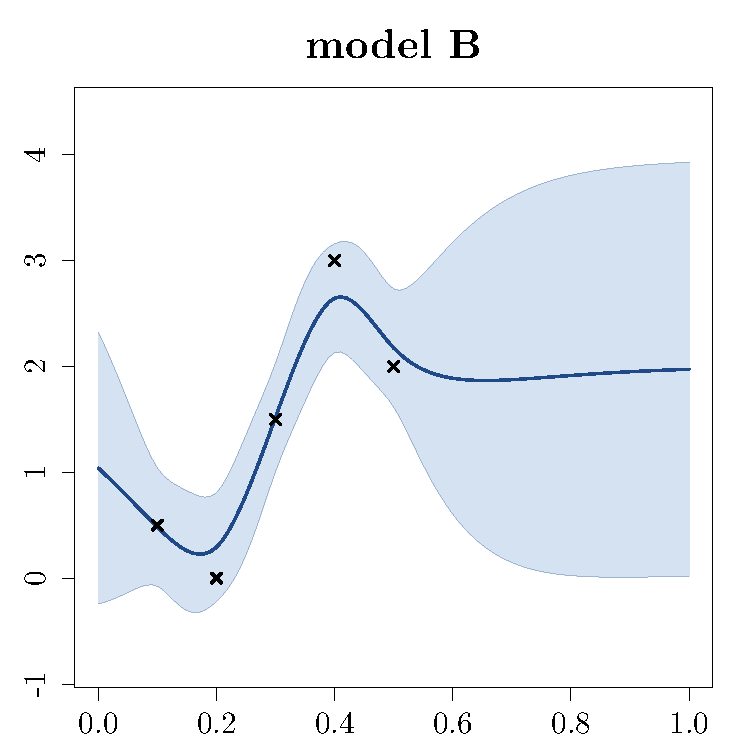
\includegraphics[width=4.6cm]{figures/exo_kriging_5.pdf}\quad 
  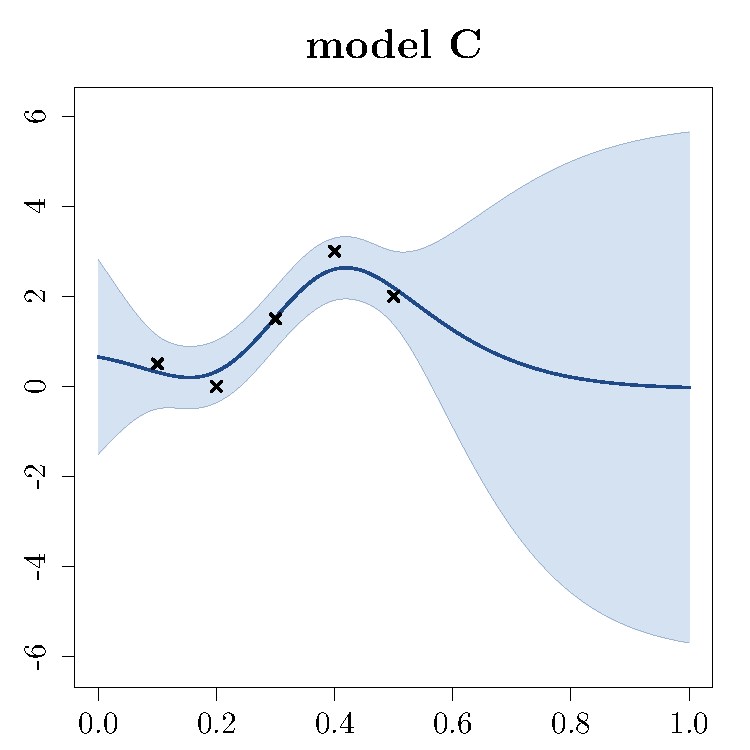
\includegraphics[width=4.6cm]{figures/exo_kriging_1.pdf}\\ \ \\
  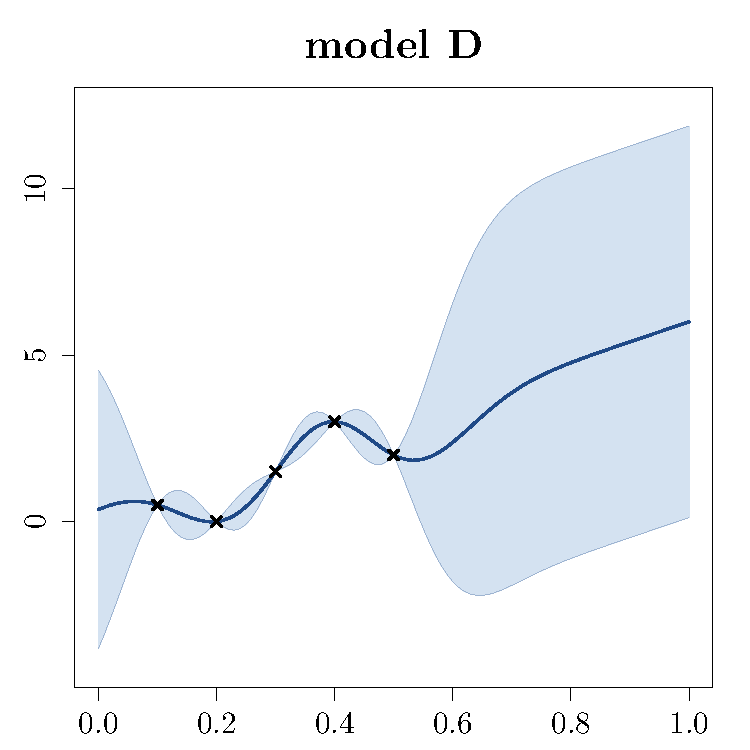
\includegraphics[width=4.6cm]{figures/exo_kriging_2.pdf}\quad 
  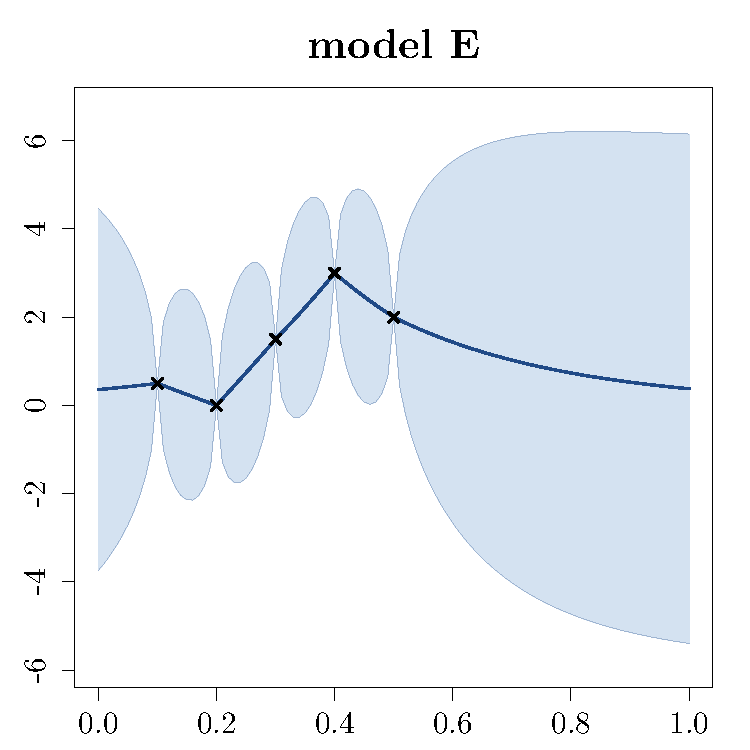
\includegraphics[width=4.6cm]{figures/exo_kriging_4.pdf}\quad 
  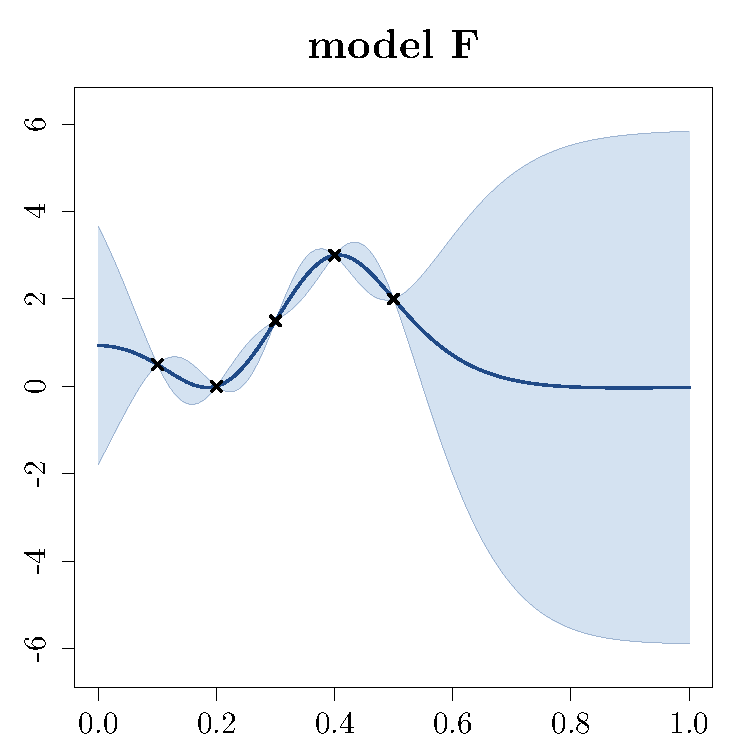
\includegraphics[width=4.6cm]{figures/exo_kriging_6.pdf}
\end{center}
\medskip
\begin{enumerate}[label=Q\arabic*.]
\item[\textbf{bonus:}] Regarding the plot of model \emph{D}, can you specify if the prediction type is \emph{simple}, \emph{ordinary} or \emph{universal kriging}?
\end{enumerate}

%%%%%%%%%%%%%%%%%%%%%%%%%%%%%%%%%%%%%%%%%%%%%%%%%%%%%%%%%%%%%%%%%%%%
%%%%%%%%%%%%%%%%%%%%%%%%%%%%%%%%%%%%%%%%%%%%%%%%%%%%%%%%%%%%%%%%%%%%
\subsection*{Exercise 5: Kernel design \hfill [7 pts]}
\begin{center}
  \emph{All the questions from this exercise may be treated independently.}
\end{center}
We consider the following kernel for $x,\ y \in \mathds{R} $:
% \begin{equation*}
%  k(x,y) = 
%  \underbrace{\sigma_0^2 \vphantom{\left(\frac{(y)^2}{2^2}\right)}}_{k_0(x,y)} +
%  \underbrace{\sigma_1^2 xy \vphantom{\left(\frac{(y)^2}{2^2}\right)}}_{k_1(x,y)} + 
%  \underbrace{\sigma_2^2 x^2y^2 \vphantom{\left(\frac{(y)^2}{2^2} \right)}}_{k_2(x,y)} + 
%  \underbrace{\sigma_3^2 \exp \left(-\frac{(x-y)^2}{2 \theta^2} \right)}_{k_3(x,y)}\, .
% \end{equation*}

\begin{align*}
 k(x,y)= k_0(x,y) + k_1(x,y) + k_2(x,y) + k_3(x,y)
\end{align*}
\begin{align*}
 \text{\qquad \qquad where \qquad} k_0(x,y)&=\sigma_0^2   &  k_1(x,y)&=\sigma_1^2 xy \\
 k_2(x,y)&= \sigma_2^2 x^2y^2 & k_3(x,y)&=\sigma_3^2 \exp \left(-\frac{(x-y)^2}{2 \theta^2} \right) .
\end{align*}

\begin{enumerate}[label=Q\arabic*.]
\item {[1 pt]} Show that $k$ is a valid covariance function. You can use the fact that the kernels in Table 1.1 from page 14 of the lecture notes are valid covariance functions without proving it. 
\item {[1 pt]} Write a \emph{R} function (you may choose another language if you prefer) that takes as inputs two vectors (say $a$, $b$) and a variance parameter $s2$ and that returns the covariance matrix with general term $k_2(a_i,b_j)$.
\item {[2 pts]} Let $Z$ be a centred Gaussian process with covariance $k$. Show carefully that $Z$ has the same distribution as the sum of 4 independent Gaussian processes:
\begin{equation*}
Z_0 \sim \mathcal{N}(0,k_0)\, ,\ 
Z_1 \sim \mathcal{N}(0,k_1)\, ,\ 
Z_2 \sim \mathcal{N}(0,k_2)\text{ and } 
Z_3 \sim \mathcal{N}( 0,k_3).
\end{equation*}
Represent graphically (for $x \in [-1,1]$) a typical sample from each of this processes for the following parameters values: $\sigma_i^2 = 1$ and $\theta = 0.2$.
\item {[1 pt]} let $(X,Y)$ be a set of $n$ observation points. What is the expression of the conditional mean and variance of $Z(x)$ given $Z(X)=F$. How does the mean function behaves when the prediction point $x$ is far away from the observations $X$?
\item {[2 pts]} Show that the conditional mean writes as a sum of conditional mean functions : $m(x) = m_0 + \dots + m_3(x)$. According to this, what is the polynomial content $m_p$ of the mean function $m$? What is the conditional variance that can be associated to $m_p$?
\item[\textbf{bonus:}] Would we obtain the exact same model as $m$ if we were to construct a universal kriging model with kernel $k_3$ and a trend of the form $\beta_0 + \beta_1 x + \beta_2 x^2$?
\end{enumerate}

%%%%%%%%%%%%%%%%%%%%%%%%%%%%%%%%%%%%%%%%%%%%%%%%%%%%%%%%%%%%%%%%%%%%
%%%%%%%%%%%%%%%%%%%%%%%%%%%%%%%%%%%%%%%%%%%%%%%%%%%%%%%%%%%%%%%%%%%%
\subsection*{Exercise 6: Optimization \hfill [3 pts]}

Consider a kriging model based on the design of experiments $X=(-0.2,0.2)$ and the vector of observations $Y=(-0.2,0.2)$. We will consider fixed values for the variance and length-scale parameters: $\sigma^2=1$ and $\theta=0.2$.
\begin{enumerate}[label=Q\arabic*.]
\item {[1 pt]} Use simple kriging equations with exponential covariance kernel to get
  the prediction at \(x=0\). We recall the inversion formula for a $2 \times 2$ matrix:
  \begin{equation}
  \left[ \begin{array}{ccc}  a & b \\ b & a   \end{array} \right] ^{-1} = \frac{1}{a^2-b^2} \times \left[ \begin{array}{ccc}  a & -b \\ -b & a   \end{array} \right]
  \end{equation}
\item {[1 pt]} Evaluate the Expected Improvement criterion at \(x=0\). The figure bellow may be helpful.
\item {[1 pt]} The same evaluation for a model based on a Gaussian kernel gives $EI(0) = 0.15$. Compare with the previous result and analyse.
  \end{enumerate}

\begin{center}
  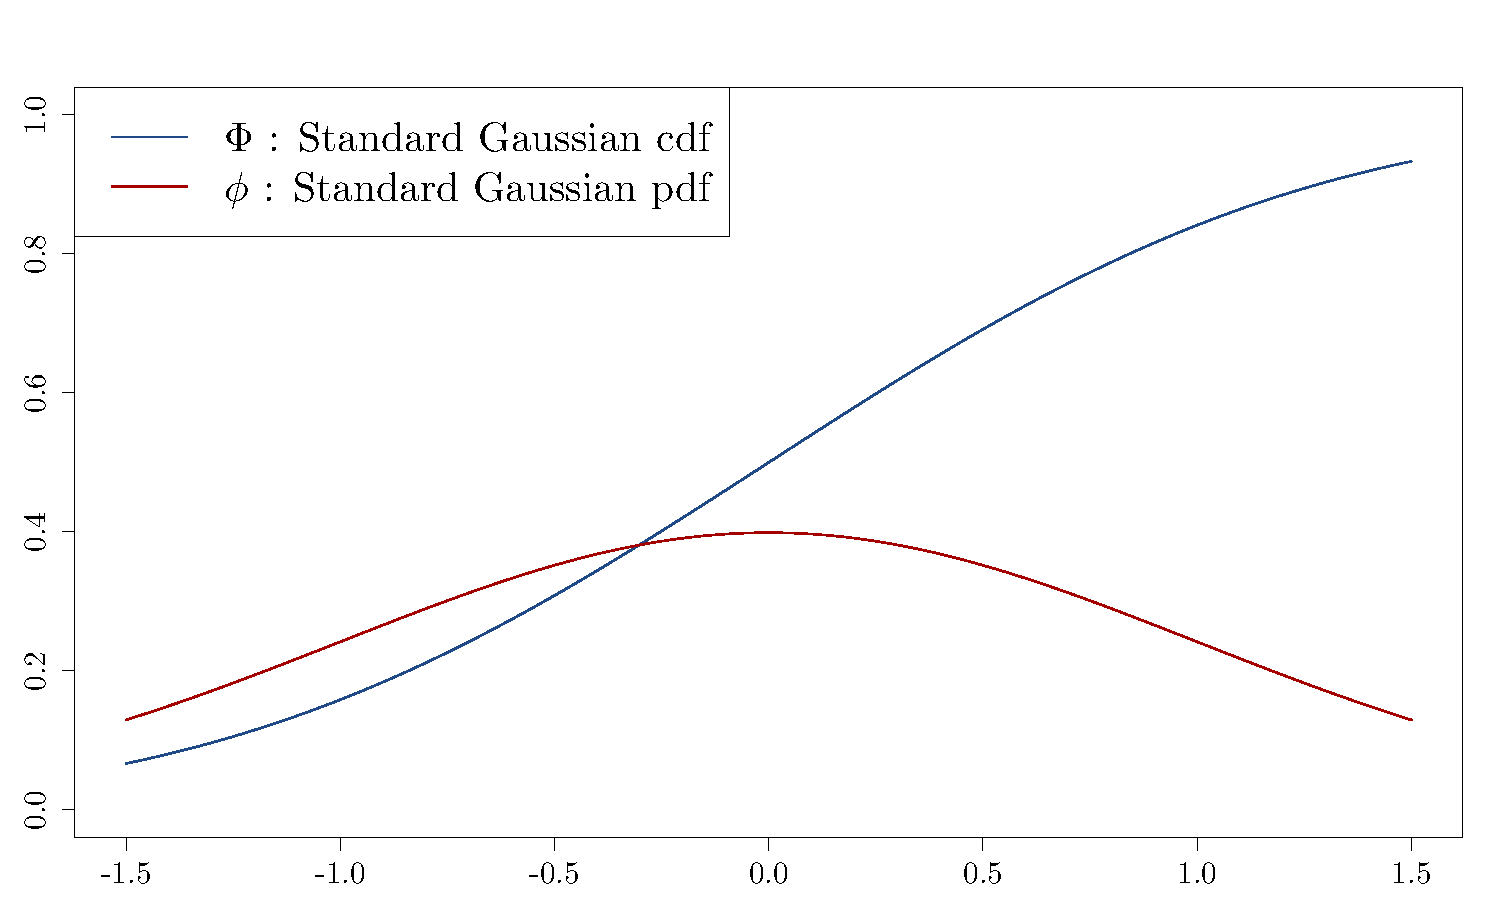
\includegraphics[width=12cm]{figures/exo_optim.pdf}
\end{center}

\end{document}











Given 
\begin{itemize}
	\item the kernel (either exponential, Brownian, squared exponential or Mat\'ern 3/2),
	\item if the process is centred (yes/no),
	\item if the process is stationary (yes/no).
\end{itemize}
\begin{center}
	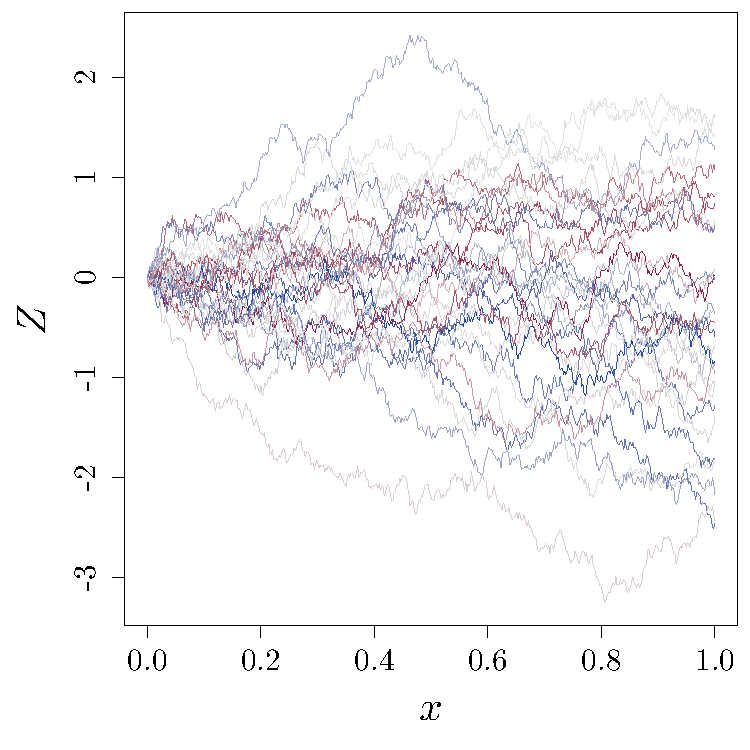
\includegraphics[width=5cm]{figures/GPR_simBrown.pdf} \qquad
	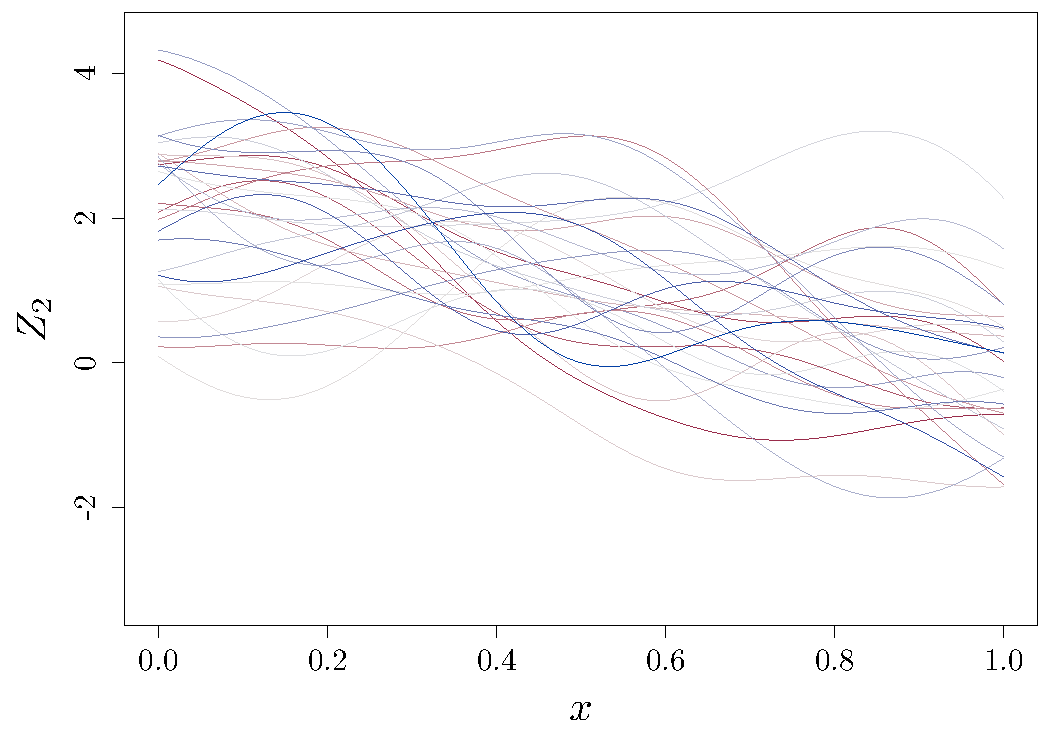
\includegraphics[width=5cm]{figures/GPR_simGauss.pdf}\\
	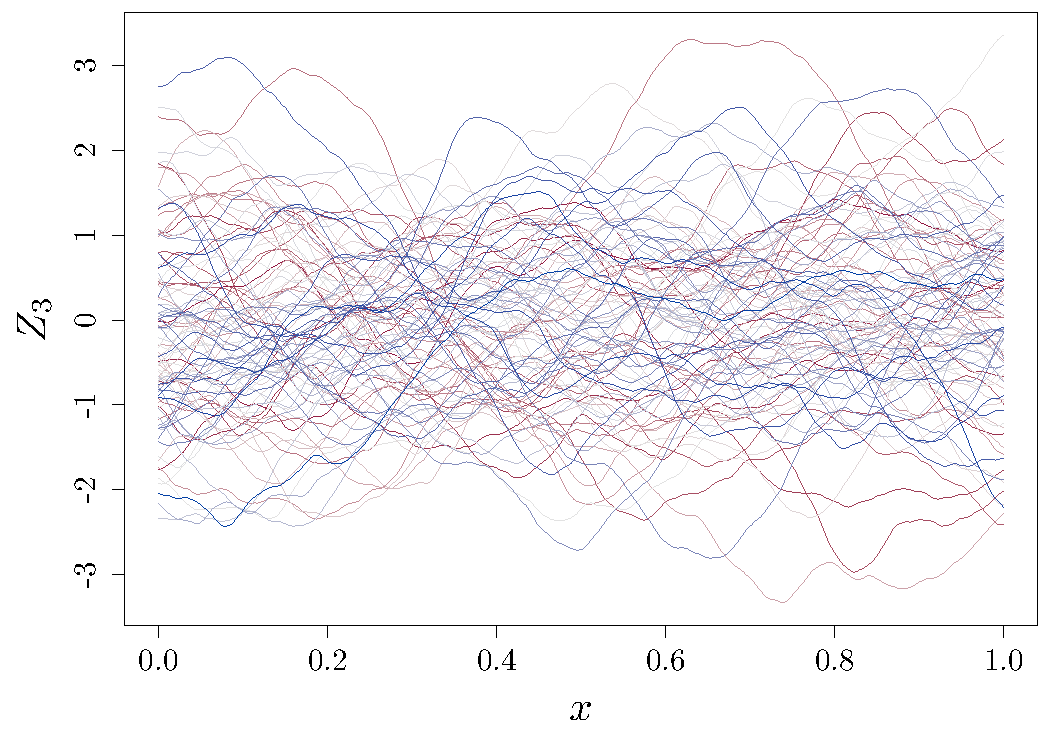
\includegraphics[width=5cm]{figures/GPR_simMat.pdf} \qquad
	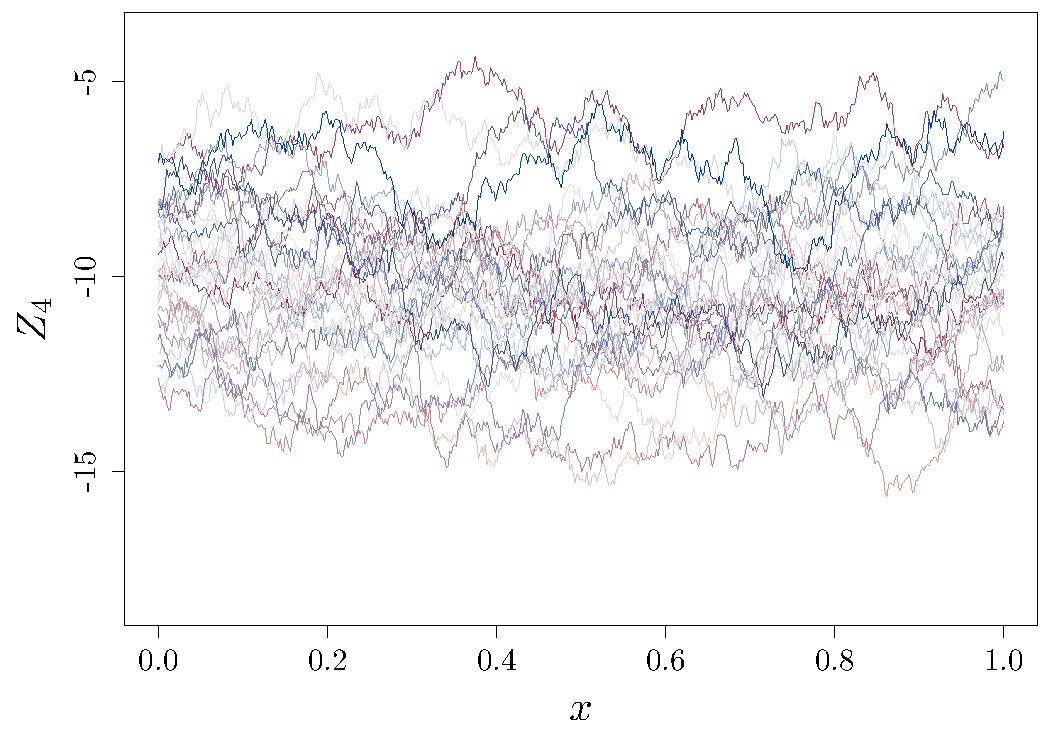
\includegraphics[width=5cm]{figures/GPR_simExp.pdf}
\end{center}
\item{[1 pt]} The figures bellow correspond to samples of a Matern 5/2 kernel with variance parameter $\sigma^2 \in \{0.1, 1, 10, 100 \}$ and with length scale $\theta \in \{0.1,1,10\}$. For each figure, specify the corresponding set of parameters.
\begin{center}
	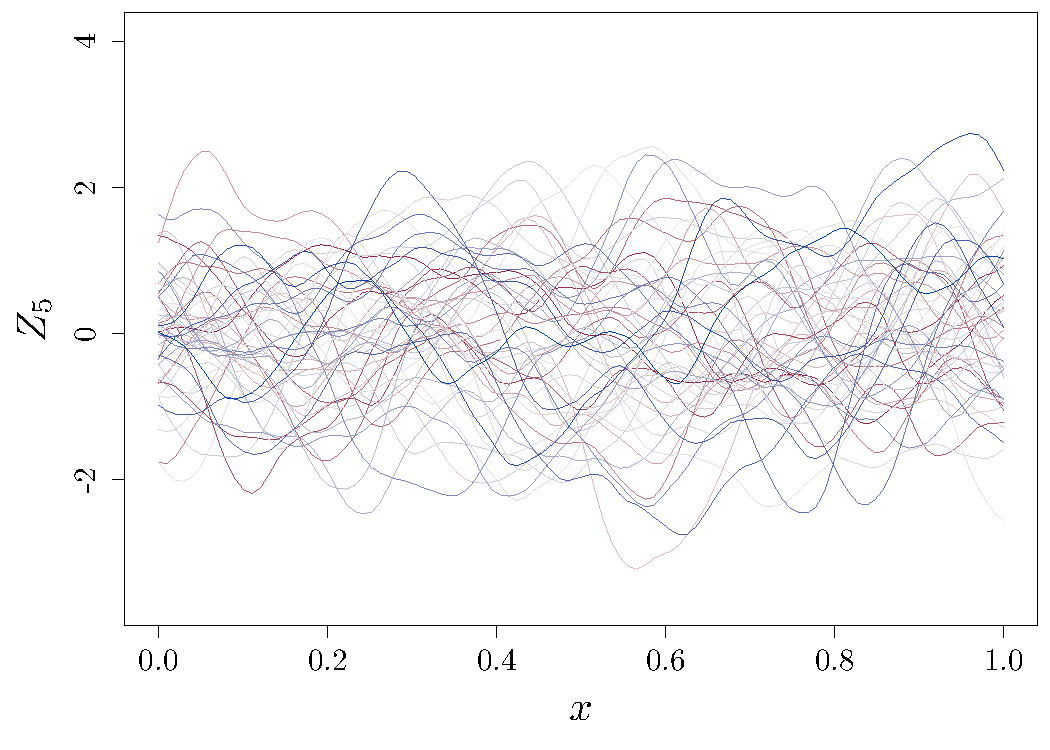
\includegraphics[width=5cm]{figures/GPR_simMat52_1_01.pdf} \qquad
	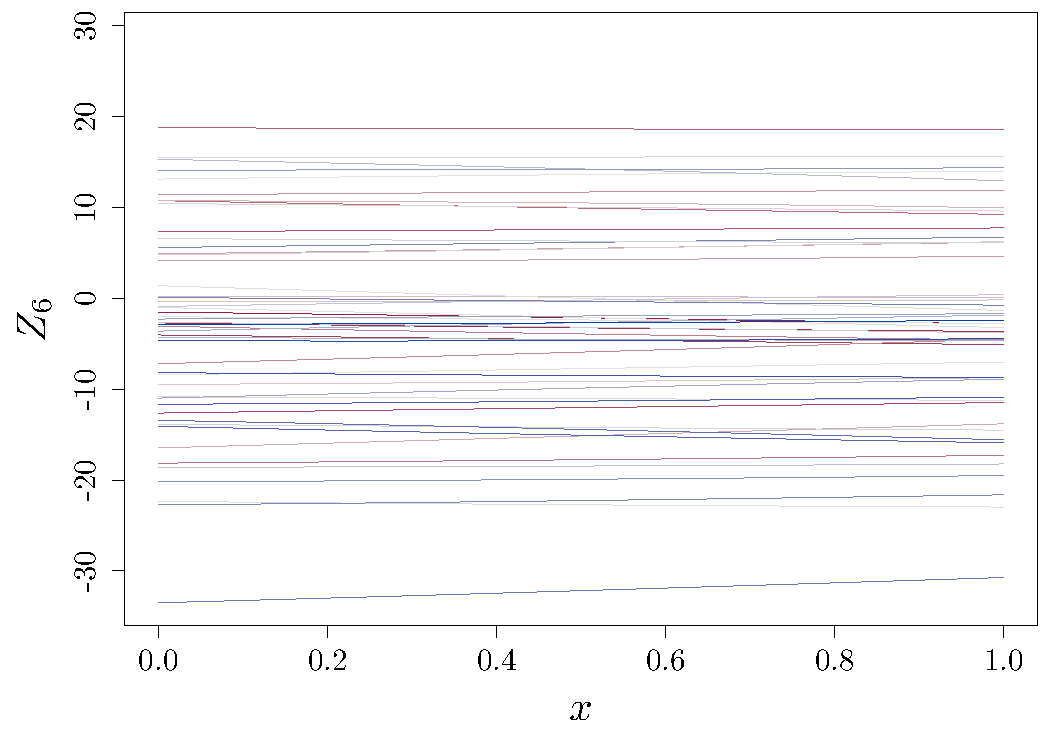
\includegraphics[width=5cm]{figures/GPR_simMat52_100_10.pdf} \\
\end{center}
\item {[1.5 pts]} We are interested in computing the mean value of a function $f$ using no more that 50 observations. What are the main steps you would go through for solving this problem.
\end{enumerate} 

\newpage
%%%%%%%%%%%%%%%%%%%%%%%%%%%%%%%%%%%%%%%%%%%%%%%%%%%%%%%%%%%%%%%%%%%%
%%%%%%%%%%%%%%%%%%%%%%%%%%%%%%%%%%%%%%%%%%%%%%%%%%%%%%%%%%%%%%%%%%%%
\section*{Exercise 2 (7 pts)}
Let us consider the 2-dimensional function: $f(x_{1},x_{2})= x_1 + x_2 + x_1 x_2$.\\

\noindent
The aim is to perform a global sensitivity analysis of $f(X_{1},X_{2})$
where $X_{1}$, $X_{2}$ are independent uniform random variables, 
with $X_1 \sim \mathcal{U} \left[-\frac{a}2,\frac{a}2 \right]$  and  $X_2 \sim \mathcal{U}[-\frac{1}2,\frac{1}2]$,
and $a>0$.\\

\noindent We recall that for a uniform random variable $Z \sim \mathcal{U}[s,t]$, 
we have $\E(Z)= \frac{s+t}2$ and $\var(Z) = \frac{(t-s)^2}{12}$.\\

\begin{enumerate}
\item {[}2 pts{]} By verifying that $X_1$, $X_2$ and $X_1X_2$ satisfy the centering and non-simplification conditions,
show that the Sobol-Hoeffding decomposition of $f(X_1, X_2)$ is simply:
$$\mu_0 = 0, \quad  \mu_1(X_1) = X_1, \quad \mu_2(X_2) = X_2, \quad \mu_{1,2}(X_1, X_2) = X_1X_2$$
\item {[}1.5 pts{]} Compute the partial variances $D_I = \var(\mu_I(X_I))$ for $I = \{1\}, \{2\}, \{1,2\}$ 
and check that the global variance is $D = \var(f(X_1, X_2)) = \frac{1}{12} \left( 1 + \frac{13}{12} a^2 \right)$ 
\item {[}1.5 pts{]} Recall that Sobol indices are defined by $S_I = D_I/D$. Compute $S_1$ and $S_2$, 
and check that $S_1$ (resp. $S_2$) is an increasing (resp. decreasing) function of $a$. Interpretation?\\
\end{enumerate} 

\noindent We now assume that $X_{1}$, $X_{2}$ are independent random variables, with $X_1, X_2 \sim \mathcal{U}[0, 1]$.\\

\begin{enumerate}
\setcounter{enumi}{3}
\item {[}0.5 pt{]} Explain why it is now \textit{wrong} that $\mu_1(X_1) = X_1$.
\item {[}1.5 pts{]} Compute the Sobol decomposition of $f(X_1, X_2)$. 
\end{enumerate}

%%%%%%%%%%%%%%%%%%%%%%%%%%%%%%%%%%%%%%%%%%%%%%%%%%%%%%%%%%%%%%%%%%%%
%%%%%%%%%%%%%%%%%%%%%%%%%%%%%%%%%%%%%%%%%%%%%%%%%%%%%%%%%%%%%%%%%%%%
\section*{Exercise 5: ANOVA kernels (8 pts)}
ANOVA kernels are kernels over $\mathds{R}^d \times \mathds{R}^d$ of the form : $ k(x,y) = \prod_{i=1}^d  \big(1+k_i(x_i,y_i) \big)$, where the $k_i$ are symmetric positive semi-definite functions.

\begin{enumerate}
\item{[1 pt]} Using the results from the course, show that ANOVA kernels are valid covariance functions.
\end{enumerate} 

\noindent We now consider costly-to-evaluate function $f: [0,1]^{10} \to \mathds{R}$, a design of experiment $X$ based on 100 points and the set of observations $F$. The knowledge we have about $f$ is that it is a smooth function that is infinitely differentiable. 

\begin{enumerate}
\setcounter{enumi}{1}
\item{[1 pt]} With such settings, which kernel would you choose and what kind of Gaussian process regression model would you consider (simple Kriging, ordinary Kriging, Universal Kriging).  
\item{[1 pt]} Give the expressions of the mean predictor and of the 95\% confidence intervals.  
\item{[1 pt]} Show that the mean predictor can be interpreted as a sum of $2^d$ functions with increasing interaction order. Does this decomposition coincides with the Sobol decomposition of the mean predictor? Why ?
\item{[1 pt]} Each term of this decomposition can be interpreted as a Gaussian process conditional distribution. Detail which one and deduce some confidence intervals associated to each sub-model.
\item{[2 pts]} According to an expert, the mean value of $f$ is 6 and the interactions of order higher than 2 can be neglected. What changes can you make in the model and in the kernel expression in order to account for these informations ?
\item{[1 pt]} We now consider a particular type for the univariate kernels $k_i$ such that $\int_0^1 k_i(s,x) \, ds = 0$ for all $x \in [0,1]$. Is there a link between the sub-models and the Sobol decomposition in this particular case?
\item[\textbf{bonus:}] Detail how to obtain a kernel $k_i$ such that $\int_0^1 k_i(s,x) \, ds = 0$ using the conditional distribution of a Gaussian process given it has zero integral.
\end{enumerate} 

Consider the kriging of following conditional points:
\[ (x,y) = \begin{cases} (-0.2,-0.2) \\\\ (0.2,0.2) \end{cases}\] with
given range \(\theta=0.2\) and variance \(\sigma^2=0.01\)

\begin{enumerate}
\def\labelenumi{\arabic{enumi}.}
\tightlist
\item
  Use simple kriging equations with exponential covariance kernel to get
  the prediction at \(x=0\).
\end{enumerate}

\textbf{Note:} \[
\left[ \begin{array}{ccc}  a & b \\ b & a   \end{array} \right] ^{-1} = {1 \over {a^2-b^2}} \times \left[ \begin{array}{ccc}  a & -b \\ -b & a   \end{array} \right]
\]

\begin{enumerate}
\def\labelenumi{\arabic{enumi}.}
\setcounter{enumi}{1}
\item
  Evaluate Expected Improvement criterion at \(x=0\).
\item
  Perform the same evaluation for gaussian kernel (with same
  parameters). Compare. Analyse.
\end{enumerate}


\end{document}
